\section{Motivation}
\label{s:background}
\label{s:nanogproblems}




\begin{figure}[t]
\begin{center}
\centering\epsfig{file=rcc/figures/nanog_table.eps, angle=270, width=\linewidth}
\end{center}
\caption{Number of threads discussing routing
  faults on the NANOG mailing list.
}
\label{tab:nanogerrors}
\end{figure}


Chapter~\ref{chap:related} (Section~\ref{sec:configuration})
describes how BGP's configuration affects which routes are originated
and propagated, how routes are modified as they propagate, which route
each router selects from multiple options, and how routes propagate
between routers.  
To understand the extent to which this complex configuration is
responsible for the types of failures that occur in practice, we studied
the archives of the North American Network Operators Group (NANOG)
mailing list, where network operators report operational problems,
discuss operational issues, etc.~\cite{nanog-list}.  Because the list
has received about 75,000 emails over the course of ten years, we first
clustered the emails by thread and pruned threads based on a list of
about fifteen keywords (\eg, ``BGP'', ``issue'', ``loop'', ``problem'',
``outage'').  We then reviewed these threads and classified each of them
into one or more of the categories shown in
Figure~\ref{tab:nanogerrors}.

This informal study shows some clear trends.  First, many routing
problems are caused by configuration faults.  Second, the same
types of problems continually appear.  Third, BGP
configuration problems continually perplex even experienced network
operators.  A tool that can detect configuration faults will clearly
benefit network operators.
